% Instructions to change to html version:
% Comment out:
%  minipage, multicols,columnbreak, mathbf, hrule
% Replace all: \begin{minipage}% %%%%\end{minipage} %%%%%%%\begin{mulicols}  %%%%%%\end{mulicols}  %%%%%\columnbreak % %%%%%\begin{framed} %%%%%%\end{framed} %%%\hrule
% Search for  
% Replace \\] with \[ and \) with \(
% Enclose graphics in figure environments and add captions
% Re-tag \df environments as sections, subsections, etc.
% Command Line Code to Create html version:
%First: pdflatex -shell-escape filename.tex                                   
%Second, for each figure: inkscape "filename-figure1.pdf" -o "filename-figure1.png"
% Third: htlatex filename.tex "ht5mjlatex.cfg, charset=utf-8" " -cunihtf -utf8"


\documentclass[10pt]{article}

%\usepackage{tikz, pgf,pgfplots,wasysym,array}
%\usepackage{wasysym}

\usepackage{amsmath,amssymb}

\ifdefined\HCode
  \def\pgfsysdriver{pgfsys-tex4ht-updated.def}
\fi 
%\ifdefined\HCode
%  \def\pgfsysdriver{pgfsys-dvisvgm4ht.def}
%\fi 
\usepackage{tikz}
\usetikzlibrary{calc,decorations.markings,arrows}
\usepackage{pgfplots}

\pgfplotsset{compat=1.12}
\usepackage{myexternalize}
%\usetikzlibrary{calc,decorations.markings,arrows}
\usepackage{framed}
\usepackage[none]{hyphenat}

\input{../../../common/1336_header_test.tex}

\begin{document}

\everymath{\displaystyle}

\renewcommand{\myTitle}{MATH 2330: Multivariable Calculus}

\renewcommand{\mySubTitle}{%Section 12.3: Double Integrals in Polar Coordinates\\
%\& 
Section 5.6: Applications of Double Integrals}
%~\hfill Name: \underline{~~~~~~~~~~~~~~~~~~~~~~~~~~~~~~~~~~~~~~~~~~~~~~~}

\lectTitle{\vspace*{-.5in}\myTitle}{\vspace*{.1in}\mySubTitle \vspace*{-.25in}}

\setlength{\columnseprule}{0.4pt}
\setlength{\columnsep}{3em}
%
%\section*{12.3: Double Integrals in Polar Coordinates}
%
%\hspace*{-.8in}%\begin{minipage}{1.25\textwidth}
%%\begin{framed}
%
%\begin{multicols}{2}
%
%\df{\textcolor{sblack}{Polar Coordinates:}}
%
%
%\includegraphics[height=2in]{Ch12s3-Polar-Coordinates}
%
%\(x=r \cos\theta, \qquad y=r\sin\theta, \qquad x^2 + y^2 = r^2\)
%
%\textbf{For the purposes of this class: \({r\geq0}\) }\\
%
%
%
%%\columnbreak
%
%\df{\textcolor{sblack}{Radially Simple Regions:}}
%
%\includegraphics[height=2in]{Ch12s3-Radially-Simple}
%
%\[
%\iint_{D} f(x,y)\ dA = \int_\alpha^\beta \int_{h_1(\theta)}^{h_2(\theta)} f(r\cos\theta,r\sin\theta)\ r\ dr\ d\theta
%\]
%
%\textbf{Area Element: \({dA = r\ dr\ d\theta}\)}\\~\\
%\textbf{Make sure that you integrate in the direction of increasing \({\theta}\) values!}
%
%
%\end{multicols}
%
%%\end{framed}
%
%%\end{minipage}
%
%
%\section*{Examples:}
%
%
%\begin{enumerate}[{Example} 1: ]
%\item Evaluate \(\iint_{R} x^2+y^2+1 \ dA\) where \({R}\) is the disk bounded by \(x^2+y^2=4\).
%
%\vfill
%
%\item Evaluate \(\iint_{R} (x^2+y^2)^2\ dA\) where \({R}\) is the ``bow tie'' region shaded below,\\
% which is bounded by \(y=x\) and \(y=-x\) and \(x^2+y^2=16\).
%
%%\begin{minipage}{.3\textwidth}
%%\hspace*{-.5in}
%\begin{tikzpicture}
%\begin{axis}[
%	y=.4cm,
%    x=.4cm,
%	axis x line=middle,
%	axis y line = middle,
%	xmin=-4,xmax=4,
%	ymin=-4,ymax=4,
%    grid=none,
%%    ticks=none,
%%    yticklabels={-5,-3,,1,3,5},
%%    xticklabels={},
%    xtick={-5,-3,3,5},
%    ytick={-5,-3,3,5},
%    xticklabels={,-4,4,},
%    yticklabels={,-4,4,},
%    xlabel=x,
%    ylabel=y,
%    label style={font=\scriptsize},
%    tick label style={font=\scriptsize}
%]
%
%\filldraw[fill=green!40,draw=green!50!black,fill opacity=.4] (axis cs: 0,0) -- (axis cs: 2.121,-2.121) arc
%(-45:45:1.2cm) -- (axis cs: 2.121,2.121) --(axis cs: 0,0) -- cycle;
%
%\filldraw[fill=green!40,draw=green!50!black,fill opacity=.4] (axis cs: 0,0) -- (axis cs: -2.121,2.121) arc
%(135:215:1.2cm) -- (axis cs: -2.121,-2.121) --(axis cs: 0,0) -- cycle;
%
%%\filldraw[fill=green!40,draw=green!50!black,fill opacity=.4] (axis cs: 0,0) -- (axis cs: 2.121,2.121) arc
%%(45:315:1.2cm) -- (axis cs: 0,0)  -- cycle;
%
%%\filldraw[fill=green!20,draw=green!50!black] (1.5cm,3.75cm) -- (3.75cm,3.75cm) arc
%%(0:45:3.75cm) -- (6.402cm,6.402cm) arc (45:0:1.5cm) -- cycle;
%
%
%\addplot +[blue, thick, dashed, mark=none, domain=-3:3, samples=100, smooth] {x};
%\addplot +[blue, thick, dashed, mark=none, domain=-3:3, samples=100, smooth] {-x};
%
%
%
%
%\end{axis}
%
%
%
%
%\end{tikzpicture}
%%\end{minipage}
%
%\vfill
%
%\item Show that \(\int_{-\infty}^\infty e^{-\frac{x^2}{2}}\ dx = \sqrt{2\pi}\).
%
%
%
%
%
%\end{enumerate}
%
%\pagebreak
%
%\section*{Section 12.3 Group Work:}
%
%\includegraphics[height=.9\textheight]{Fun-with-Polar-Volume}

%\vspace*{-.2in}
%\section*{Section 12.4: Applications of Double Integrals}

\hspace*{-.8in}%\begin{minipage}{1.25\textwidth}
%\begin{framed}

\section*{Key Concept:}

Given a \textbf{density function} \(\rho(x,y)\) that tells how much \(\frac{\text{``stuff''}}{\text{unit area}}\) there is at a given point in a region \(D\), then
\[
\iint_D \rho(x,y)\ dA
\]
calculates the ``total amount of stuff'' within region \(D\).\\~\\

Example: If \(u(x,y)\) represents the population density in region \(D\), then \(\iint_D u(x,y)\ dA\) gives the total population in region \(D\).\\~\\

%If \(\sigma(x,y)\) represents the charge density of region \(D\), then \(\iint_D u(x,y)\ dA\) gives the total charge of region \(D\).
%\hrule
\vspace*{.1in}

%\begin{multicols}{2}

\section*{Center of Mass of a Lamina:}


\includegraphics[height=2in]{Ch12s4-Lamina.png}

mass density function: \(\rho(x,y)\) has units \(\frac{\text{mass}}{\text{area}}\)\\~\\
total mass of the lamina: \(m = \iint_D \rho(x,y)\ dA\)\\~\\
Center of mass: \((\bar{x},\bar{y})\)\\~\\
\(\bar{x} = \frac{1}{m}\iint_D \rho(x,y) x\ dA\)\\~\\
\(\bar{y} = \frac{1}{m}\iint_D \rho(x,y) y\ dA\)





%\end{multicols}

%\end{framed}

%\end{minipage}


\section*{Example:}


%\begin{enumerate}[{Example} 1: ]
%\item 
Find the center of mass of the lamina \(D\) that has density function \(\rho(x,y)=x^2\), where \(D\) is the triangular region bounded by \(x=0, \quad y=x, \quad 2x+y=6\).


%\begin{minipage}{.3\textwidth}
\hspace*{-.5in}
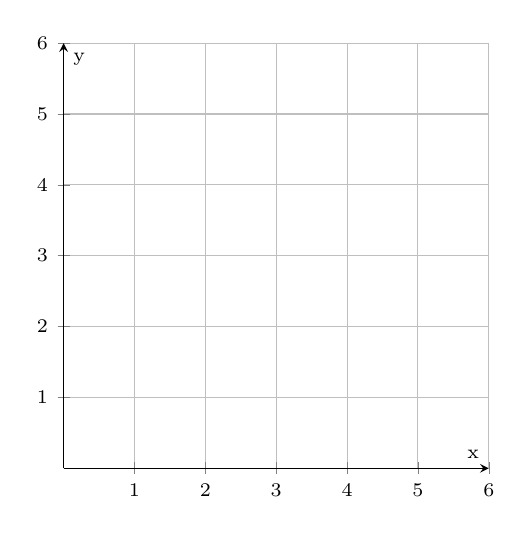
\begin{tikzpicture}
\begin{axis}[
	y=.9cm,
    x=.9cm,
	axis x line=middle,
	axis y line = middle,
	xmin=0,xmax=6,
	ymin=0,ymax=6,
    grid=both,
%    ticks=none,
%    yticklabels={-5,-3,,1,3,5},
%    xticklabels={},
    xtick={0,1,...,6},
    ytick={0,1,...,6},
    xlabel=x,
    ylabel=y,
    label style={font=\scriptsize},
    tick label style={font=\scriptsize}
]





\end{axis}




\end{tikzpicture}
%\end{minipage}

%\end{enumerate}

\end{document}

